\documentclass[12pt,a4paper]{article}
\usepackage[utf8]{inputenc}
\usepackage[brazil]{babel}
\usepackage[T1]{fontenc}
\usepackage{graphicx}
\usepackage{geometry}
\usepackage{hyperref}
\usepackage{enumitem}
\usepackage{tikz}
\usepackage{float}
\usepackage{xcolor}
\usepackage{fancyhdr}
\usepackage[most]{tcolorbox}

\geometry{margin=2.5cm}
\pagestyle{fancy}
\fancyhf{}

\renewcommand{\headrulewidth}{2pt}
\renewcommand{\footrulewidth}{2pt}

\renewcommand{\headrule}{\hbox to\headwidth{%
  \color{black}\leaders\hrule height \headrulewidth\hfill}}

\renewcommand{\footrule}{\hbox to\headwidth{%
  \color{black}\leaders\hrule height \footrulewidth\hfill}}

\setlength{\headheight}{51pt}

\fancyhead[L]{%
  
\includegraphics[height=1.2cm]{Universidade_de_Rio_Verde.jpg}
}

\fancyhead[R]{%
  \raggedleft
  \textcolor{black}{%
    \small
    \textbf{Trabalho Prático --- Árvore Geradora Mínima (Kruskal)}\\
    Me.~Sergio Souza Novak\\
    \textit{Lógica para Engenharia de Software}
  }
}

\fancyfoot[C]{%
  \textcolor{black}{\thepage}
}

\begin{document}

\begin{center}
  {\Large \textbf{Trabalho Prático: Árvore Geradora Mínima}}\\
  {\large Implementação do Algoritmo de Kruskal com Cytoscape.js}
\end{center}

\vspace{0.5cm}

\section*{Objetivo do Trabalho}

O objetivo deste trabalho prático é desenvolver uma aplicação web interativa que permita a visualização passo a passo do \textbf{Algoritmo de Kruskal} para encontrar a Árvore Geradora Mínima (MST - \textit{Minimum Spanning Tree}) de um grafo. Os alunos deverão utilizar a biblioteca \textbf{Cytoscape.js} para a renderização e manipulação visual do grafo.

\section*{Requisitos da Aplicação}

A aplicação web deve possuir uma interface dividida em duas partes principais: um painel de desenho do grafo e uma barra lateral para exibição do log de execução.

A implementação deve satisfazer os seguintes requisitos:

\begin{enumerate}
    \item \textbf{Criação de Nós e Arestas:} Deve ser possível adicionar nós clicando no painel. Arestas devem ser criadas selecionando um nó de origem e, em seguida, um nó de destino.
    \item \textbf{Pesos Automáticos e Manuais:} Ao criar uma aresta, seu peso padrão deve ser calculado como a distância euclidiana entre os dois nós. O usuário também deve poder alterar o peso de qualquer aresta clicando sobre ela, através de uma caixa de diálogo (\textit{prompt}).
    \item \textbf{Exclusão de Elementos:} Nós e arestas devem poder ser excluídos ao se clicar com o botão direito (ou toque longo) sobre eles. Ao excluir um nó, todas as suas arestas incidentes também devem ser removidas automaticamente.
    \item \textbf{Algoritmo de Kruskal Passo a Passo:} 
    \begin{itemize}
        \item A aplicação não deve apenas chamar a função pronta de Kruskal do Cytoscape para resolver o problema, mas sim implementar a lógica passo a passo, utilizando a estrutura de dados de \textbf{Conjuntos Disjuntos} (Union-Find).
        \item Ao clicar em um botão ``Executar Kruskal'', a aplicação deve processar as arestas do grafo em ordem crescente de seus pesos.
    \end{itemize}
    \item \textbf{Log de Execução (Barra Lateral):} O sistema deve possuir uma barra lateral que apresente as iterações do algoritmo:
    \begin{itemize}
        \item Exibir o conjunto de arestas da árvore ($A$) no início (vazio) e seu estado em cada iteração.
        \item Exibir os conjuntos auxiliares de vértices (do algoritmo Union-Find) no início e como eles se unem a cada iteração.
        \item O detalhamento de cada aresta analisada, informando claramente se a aresta foi adicionada ao conjunto $A$ (pois os vértices estavam em componentes distintos) ou se foi descartada (pois formaria um ciclo).
    \end{itemize}
\end{enumerate}

\section*{Exemplos Visuais da Interface}

Abaixo encontram-se exemplos visuais da interface esperada, mostrando a área de modelagem do grafo e os logs de iteração do algoritmo na barra lateral.

\begin{figure}[htbp]
    \centering
    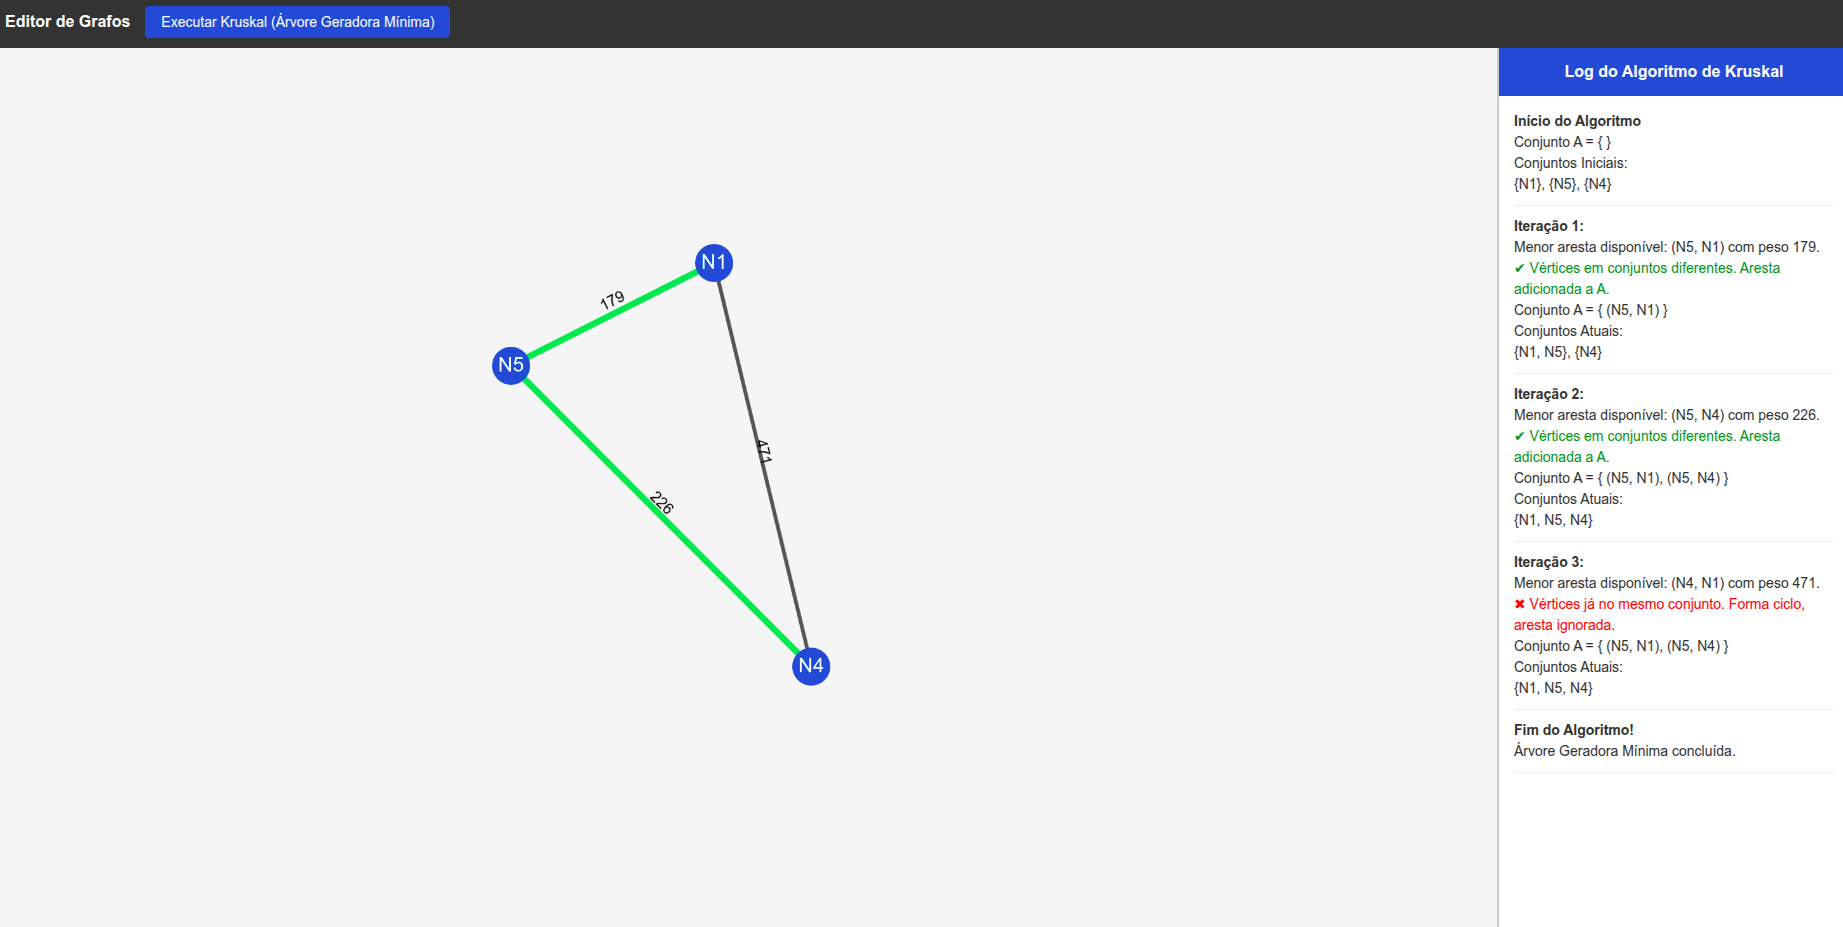
\includegraphics[width=0.8\textwidth]{image.png}
    \caption{Exemplo da interface com o grafo construído sendo editado pelo usuário.}
    \label{fig:interface1}
\end{figure}

\begin{figure}[htbp]
    \centering
    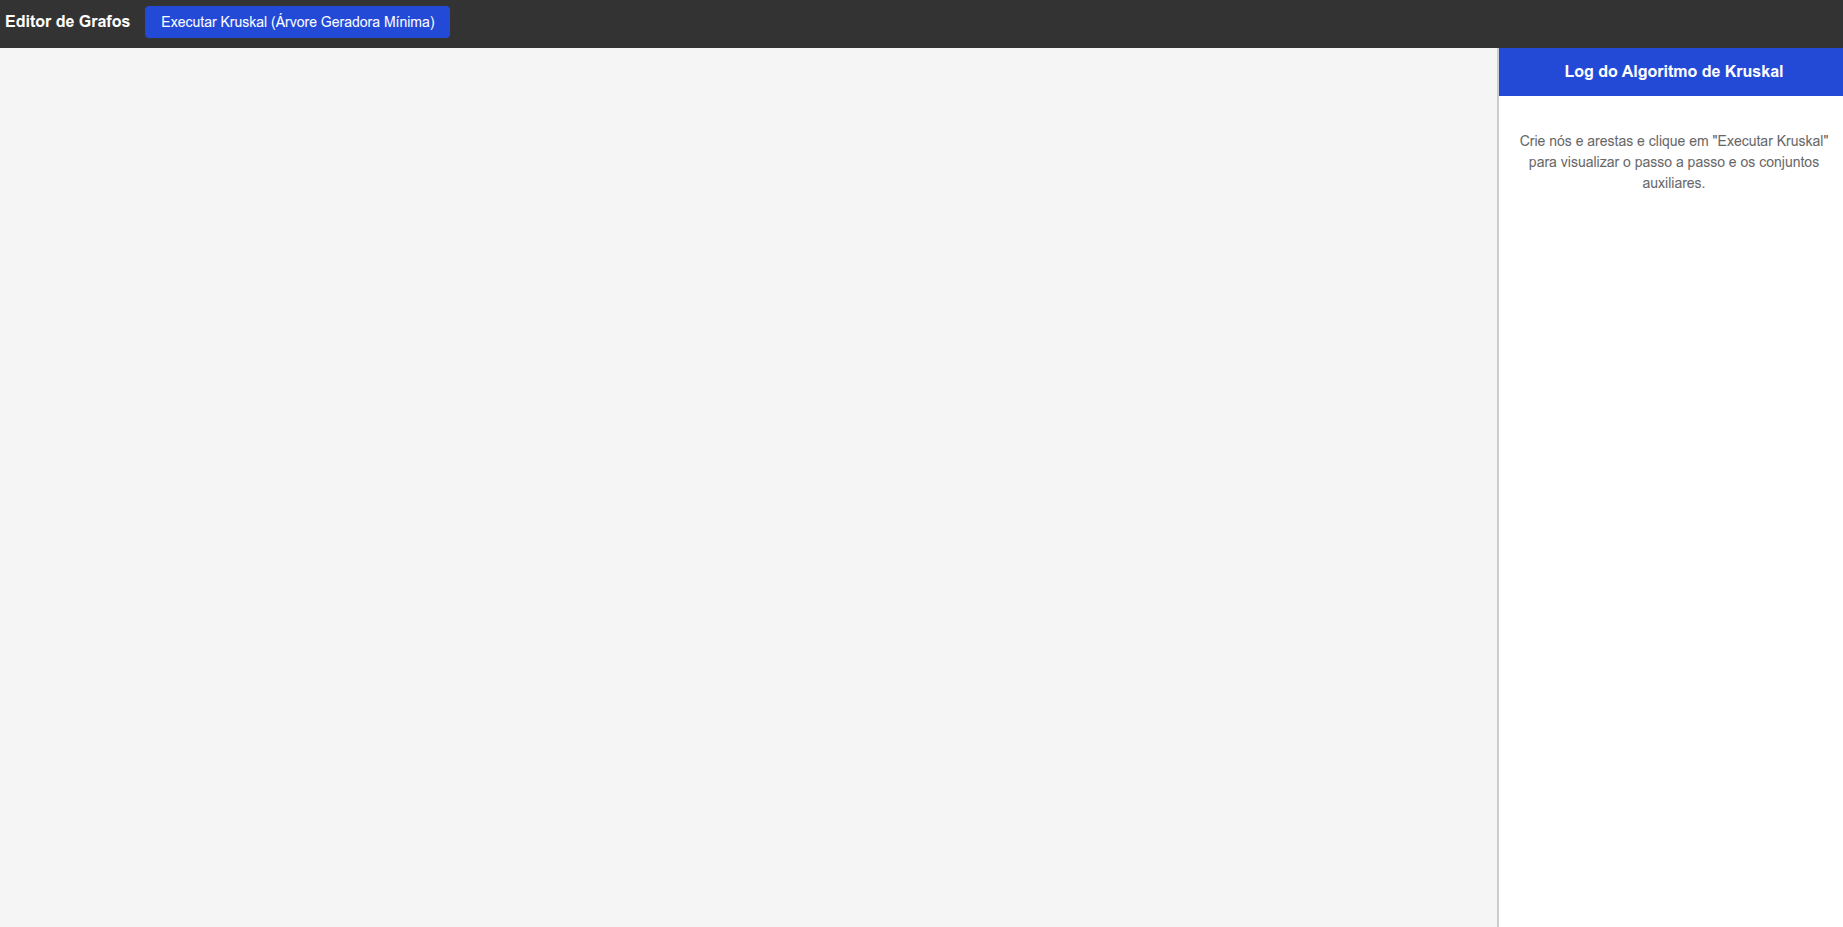
\includegraphics[width=0.8\textwidth]{image2.png}
    \caption{Execução do Algoritmo de Kruskal, exibindo a Árvore Geradora Mínima destacada no grafo.}
    \label{fig:interface2}
\end{figure}

\begin{figure}[htbp]
    \centering
    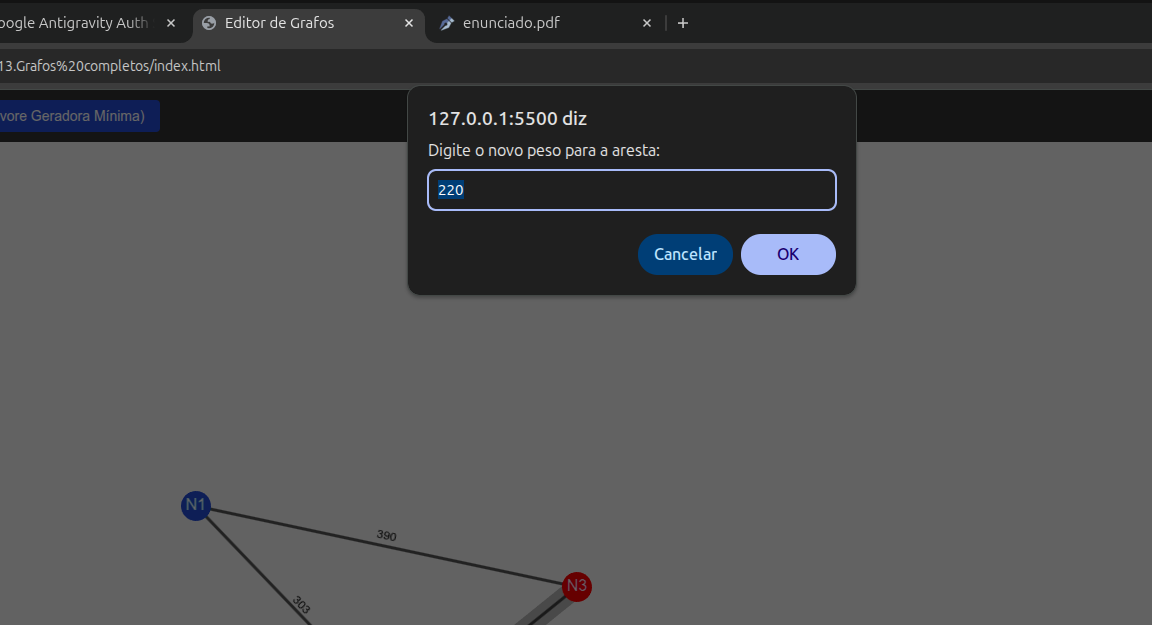
\includegraphics[width=0.8\textwidth]{image3.png}
    \caption{Edição manual do peso de uma aresta após clique no elemento.}
    \label{fig:interface3}
\end{figure}

\begin{figure}[htbp]
    \centering
    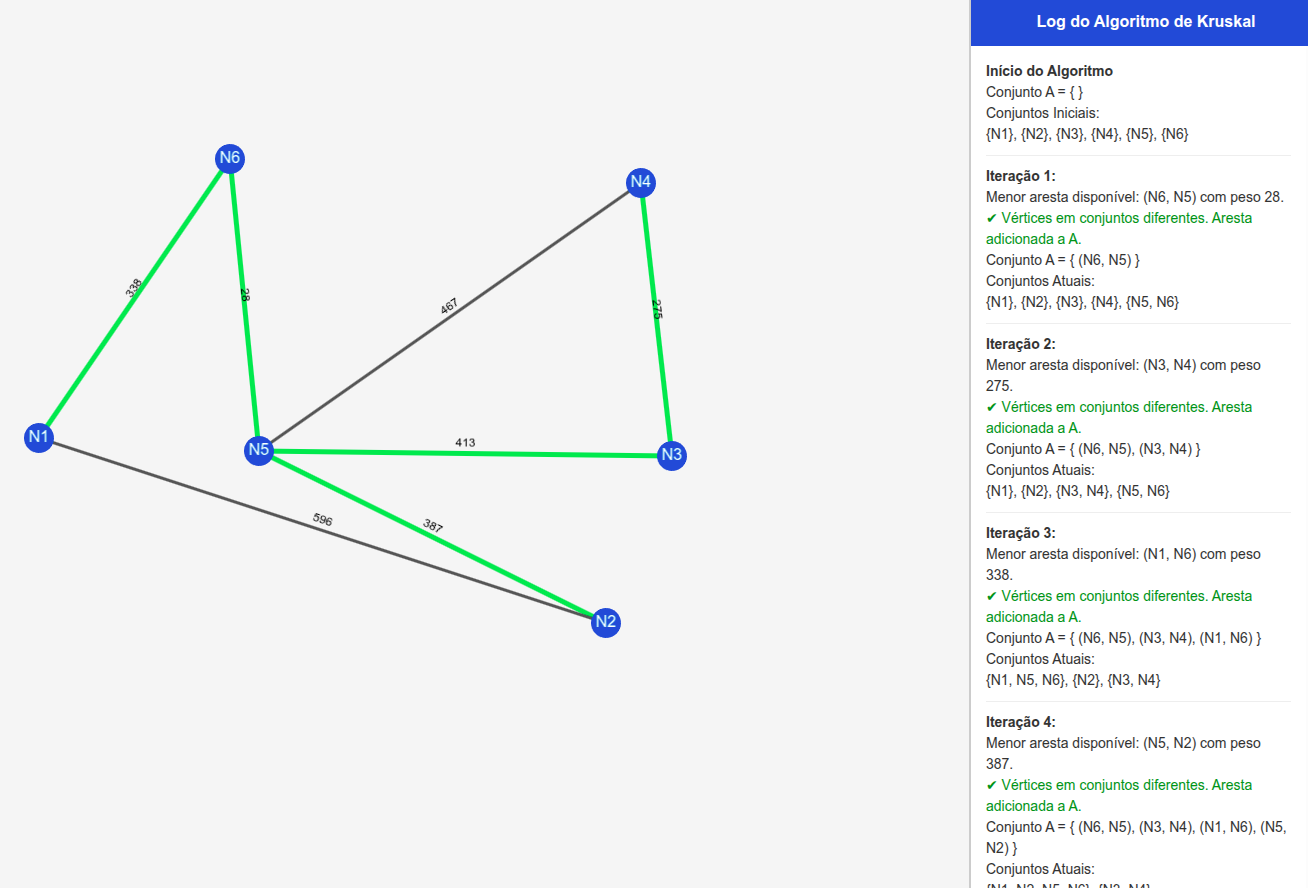
\includegraphics[width=0.8\textwidth]{image4.png}
    \caption{Outra parte da execução, mostrando os conjuntos disjuntos e o conjunto A passo a passo.}
    \label{fig:interface4}
\end{figure}

\begin{figure}[htbp]
    \centering
    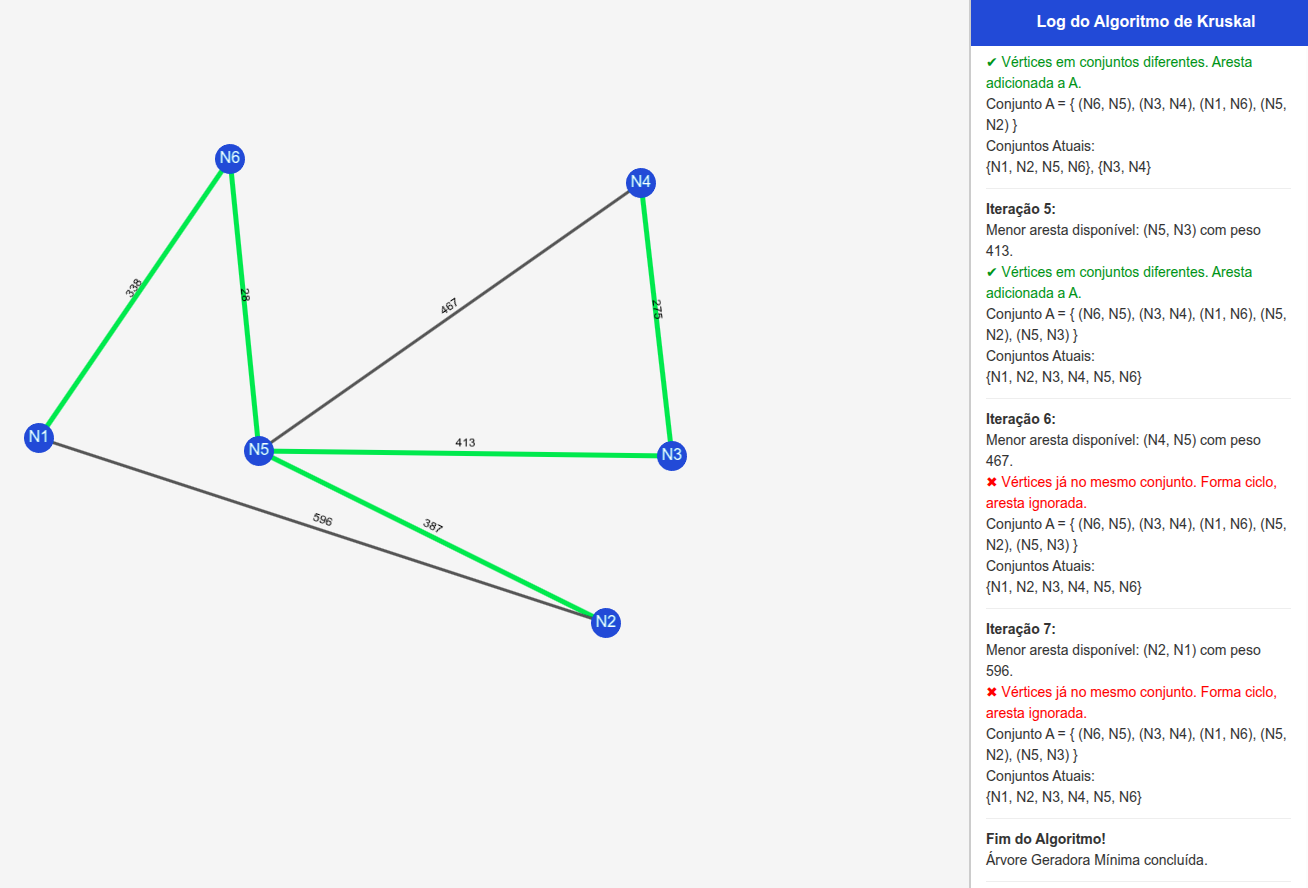
\includegraphics[width=0.8\textwidth]{image5.png}
    \caption{Detalhe do log de execução concluído.}
    \label{fig:interface5}
\end{figure}

\section*{Exemplo do Log de Execução}

Para garantir que a formatação da barra lateral atenda aos requisitos, a saída gerada a cada execução deve seguir o formato textual exemplificado abaixo (a interface real pode usar estilos HTML/CSS para deixar mais legível, com cores indicando sucesso ou falha).

\begin{verbatim}
Início do Algoritmo
Conjunto A = { }
Conjuntos Iniciais:
{N1}, {N2}, {N3}, {N4}, {N5}, {N6}

Iteração 1:
Menor aresta disponível: (N6, N5) com peso 28.
 Vértices em conjuntos diferentes. Aresta adicionada a A.
Conjunto A = { (N6, N5) }
Conjuntos Atuais:
{N1}, {N2}, {N3}, {N4}, {N5, N6}

Iteração 2:
Menor aresta disponível: (N3, N4) com peso 275.
 Vértices em conjuntos diferentes. Aresta adicionada a A.
Conjunto A = { (N6, N5), (N3, N4) }
Conjuntos Atuais:
{N1}, {N2}, {N3, N4}, {N5, N6}

Iteração 3:
Menor aresta disponível: (N1, N6) com peso 338.
 Vértices em conjuntos diferentes. Aresta adicionada a A.
Conjunto A = { (N6, N5), (N3, N4), (N1, N6) }
Conjuntos Atuais:
{N1, N5, N6}, {N2}, {N3, N4}

Iteração 4:
Menor aresta disponível: (N5, N2) com peso 387.
 Vértices em conjuntos diferentes. Aresta adicionada a A.
Conjunto A = { (N6, N5), (N3, N4), (N1, N6), (N5, N2) }
Conjuntos Atuais:
{N1, N2, N5, N6}, {N3, N4}

Iteração 5:
Menor aresta disponível: (N5, N3) com peso 413.
 Vértices em conjuntos diferentes. Aresta adicionada a A.
Conjunto A = { (N6, N5), (N3, N4), (N1, N6), (N5, N2), (N5, N3) }
Conjuntos Atuais:
{N1, N2, N3, N4, N5, N6}

Iteração 6:
Menor aresta disponível: (N4, N5) com peso 467.
 Vértices já no mesmo conjunto. Forma ciclo, aresta ignorada.
Conjunto A = { (N6, N5), (N3, N4), (N1, N6), (N5, N2), (N5, N3) }
Conjuntos Atuais:
{N1, N2, N3, N4, N5, N6}

Iteração 7:
Menor aresta disponível: (N2, N1) com peso 596.
 Vértices já no mesmo conjunto. Forma ciclo, aresta ignorada.
Conjunto A = { (N6, N5), (N3, N4), (N1, N6), (N5, N2), (N5, N3) }
Conjuntos Atuais:
{N1, N2, N3, N4, N5, N6}

Fim do Algoritmo!
Árvore Geradora Mínima concluída.
\end{verbatim}

\section*{Entrega: Vídeo Explicativo}

Além do código-fonte, o aluno deverá gravar e entregar um \textbf{vídeo explicativo} demonstrando o funcionamento da aplicação. O vídeo deve cobrir obrigatoriamente os seguintes casos:

\begin{enumerate}
    \item \textbf{Grafo Completo $K_5$} -- grafo com 5 vértices onde todo par de vértices possui uma aresta (10 arestas no total). O aluno deve construir o grafo, atribuir pesos e executar o Kruskal, explicando cada iteração do log.
    \item \textbf{Grafo Bipartido Completo $K_{3,3}$} -- grafo com dois grupos de 3 vértices, onde cada vértice de um grupo está ligado a todos os vértices do outro grupo (9 arestas). O aluno deve demonstrar a execução do Kruskal destacando a estrutura bipartida.
    \item \textbf{Grafo com Duas Componentes Conexas} -- grafo em que os vértices estão divididos em dois grupos desconectados entre si. O aluno deve demonstrar que o algoritmo de Kruskal produz \textbf{florestas geradoras mínimas}, uma por componente, e explicar o comportamento do log nesse caso.
    \item \textbf{Grafo Completo $K_4$} -- grafo com 4 vértices e todos conectados entre si (6 arestas). O aluno deve executar o Kruskal e identificar no log quais arestas foram ignoradas por formarem ciclos.
\end{enumerate}

O vídeo deve ter no mínimo \textbf{5 minutos} e o aluno deve narrar em voz própria, explicando os conceitos do algoritmo enquanto demonstra cada grafo na aplicação.

\section*{Wireframes das Telas Esperadas}

As figuras abaixo apresentam os wireframes das telas que devem ser reproduzidas no vídeo, ilustrando a estrutura de cada grafo e o estado esperado da interface.

% ============================================================
% WIREFRAME 1 - Grafo K5
% ============================================================
\begin{figure}[H]
\centering
\begin{tikzpicture}[scale=1.3,
    node/.style={circle, draw=blue!70, fill=blue!60, text=white, font=\small\bfseries, minimum size=0.8cm},
    mstedge/.style={line width=2pt, green!60!black},
    normaledge/.style={gray, thin}
]
% Navbar
\fill[black!80] (-1,5.5) rectangle (12,6.3);
\node[white, font=\small] at (0.5,5.9) {Editor de Grafos};
\fill[blue!70] (2.5,5.6) rectangle (6.5,6.2);
\node[white, font=\tiny] at (4.5,5.9) {Executar Kruskal (MST)};
% Sidebar
\fill[blue!60] (8.5,5.5) rectangle (12,6.3);
\node[white, font=\small\bfseries] at (10.25,5.9) {Log do Algoritmo};
\fill[white] (8.5,-0.5) rectangle (12,5.5);
\draw[black!30] (8.5,-0.5) rectangle (12,5.5);
\node[font=\tiny, align=left, anchor=north west] at (8.6,5.4) {\textbf{Início:} A = \{\}\\Conj.: \{N1\},\{N2\},\{N3\},\{N4\},\{N5\}\\\\\textbf{It. 1:} (N1,N2), p=100\\+ Adicionada a A.\\A=\{(N1,N2)\}\\\\\textbf{It. 2:} (N2,N3), p=140\\+ Adicionada a A.\\\\\textbf{It. 3:} (N3,N4), p=160\\+ Adicionada a A.\\\\\textbf{It. 4:} (N4,N5), p=180\\+ Adicionada a A.\\\\\textbf{It. 5:} (N1,N3), p=200\\x Ciclo, ignorada.\\\\\textbf{Fim do Algoritmo!}};
% Nós K5 em pentágono
\coordinate (N1) at (3.5,4.5);
\coordinate (N2) at (1.5,2.8);
\coordinate (N3) at (2.3,0.5);
\coordinate (N4) at (4.7,0.5);
\coordinate (N5) at (5.5,2.8);
% Arestas normais
\draw[normaledge] (N1)--(N3); \draw[normaledge] (N1)--(N4);
\draw[normaledge] (N2)--(N4); \draw[normaledge] (N2)--(N5);
\draw[normaledge] (N3)--(N5); \draw[normaledge] (N1)--(N5); 
% Arestas MST em verde
\draw[mstedge] (N1)--(N2); \draw[mstedge] (N2)--(N3);
\draw[mstedge] (N3)--(N4); \draw[mstedge] (N4)--(N5);
% Rótulos de pesos (MST)
\node[font=\tiny, fill=white, inner sep=1pt] at (2.5,3.8) {100};
\node[font=\tiny, fill=white, inner sep=1pt] at (1.7,1.6) {140};
\node[font=\tiny, fill=white, inner sep=1pt] at (3.5,0.5) {160};
\node[font=\tiny, fill=white, inner sep=1pt] at (5.3,1.6) {180};
% Rótulos de pesos (não-MST)
\node[font=\tiny, fill=white, inner sep=1pt] at (2.9,2.5) {200};
\node[font=\tiny, fill=white, inner sep=1pt] at (4.1,2.5) {220};
\node[font=\tiny, fill=white, inner sep=1pt] at (3.1,1.65) {240};
\node[font=\tiny, fill=white, inner sep=1pt] at (3.5,2.8) {260};
\node[font=\tiny, fill=white, inner sep=1pt] at (3.9,1.65) {280};
\node[font=\tiny, fill=white, inner sep=1pt] at (4.5,3.65) {300};
% Nós
\node[node] at (N1) {N1}; \node[node] at (N2) {N2};
\node[node] at (N3) {N3}; \node[node] at (N4) {N4}; \node[node] at (N5) {N5};
% Borda
\draw[black!40] (-1,-0.5) rectangle (12,6.3);
\end{tikzpicture}
\caption{Wireframe -- Grafo Completo $K_5$ com MST destacada (arestas verdes).}
\label{fig:wire-k5}
\end{figure}

% ============================================================
% WIREFRAME 2 - Grafo Bipartido K3,3
% ============================================================
\begin{figure}[H]
\centering
\begin{tikzpicture}[scale=1.3,
    node/.style={circle, draw=blue!70, fill=blue!60, text=white, font=\small\bfseries, minimum size=0.8cm},
    mstedge/.style={line width=2pt, green!60!black},
    normaledge/.style={gray, thin}
]
% Navbar
\fill[black!80] (-1,5.0) rectangle (12,5.8);
\node[white, font=\small] at (0.5,5.4) {Editor de Grafos};
\fill[blue!70] (2.5,5.1) rectangle (6.5,5.7);
\node[white, font=\tiny] at (4.5,5.4) {Executar Kruskal (MST)};
% Sidebar
\fill[blue!60] (8.5,5.0) rectangle (12,5.8);
\node[white, font=\small\bfseries] at (10.25,5.4) {Log do Algoritmo};
\fill[white] (8.5,-0.5) rectangle (12,5.0);
\draw[black!30] (8.5,-0.5) rectangle (12,5.0);
\node[font=\tiny, align=left, anchor=north west] at (8.6,4.9) {\textbf{Início:} A = \{\}\\Conj.: \{A1\},\{A2\},\{A3\}\\\{B1\},\{B2\},\{B3\}\\\\\textbf{It. 1:} (A1,B1), p=120\\+ Adicionada a A.\\\\\textbf{It. 2:} (A2,B2), p=150\\+ Adicionada a A.\\\\\textbf{It. 3:} (A3,B3), p=170\\+ Adicionada a A.\\\\\textbf{It. 4:} (A1,B2), p=200\\+ Adicionada a A.\\\\\textbf{It. 5:} (A2,B1), p=220\\x Ciclo, ignorada.\\\\\textbf{It. 6:} (A3,B1), p=250\\x Ciclo, ignorada.\\\\\textbf{Fim do Algoritmo!}};
% Grupo A (esquerda), Grupo B (direita)
\coordinate (A1) at (2.0,4.0); \coordinate (A2) at (2.0,2.2); \coordinate (A3) at (2.0,0.4);
\coordinate (B1) at (6.0,4.0); \coordinate (B2) at (6.0,2.2); \coordinate (B3) at (6.0,0.4);
% Arestas normais
\draw[normaledge] (A1)--(B2); \draw[normaledge] (A1)--(B3);
\draw[normaledge] (A2)--(B1); \draw[normaledge] (A2)--(B3);
\draw[normaledge] (A3)--(B1); \draw[normaledge] (A3)--(B2);
% Arestas MST
\draw[mstedge] (A1)--(B1); \draw[mstedge] (A2)--(B2);
\draw[mstedge] (A3)--(B3); \draw[mstedge] (A1)--(B2);
% Rótulos (MST)
\node[font=\tiny, fill=white, inner sep=1pt] at (4.0,4.0) {120};
\node[font=\tiny, fill=white, inner sep=1pt] at (4.0,2.2) {150};
\node[font=\tiny, fill=white, inner sep=1pt] at (4.0,0.4) {170};
\node[font=\tiny, fill=white, inner sep=1pt] at (3.0,3.3) {200};
% Rótulos (Não-MST)
\node[font=\tiny, fill=white, inner sep=1pt] at (3.0,1.3) {280};
\node[font=\tiny, fill=white, inner sep=1pt] at (5.0,3.1) {220};
\node[font=\tiny, fill=white, inner sep=1pt] at (5.0,1.3) {290};
\node[font=\tiny, fill=white, inner sep=1pt] at (3.0,2.8) {250};
\node[font=\tiny, fill=white, inner sep=1pt] at (5.0,0.8) {300};
% Nós
\node[node] at (A1) {A1}; \node[node] at (A2) {A2}; \node[node] at (A3) {A3};
\node[node] at (B1) {B1}; \node[node] at (B2) {B2}; \node[node] at (B3) {B3};
% Borda
\draw[black!40] (-1,-0.5) rectangle (12,5.8);
\end{tikzpicture}
\caption{Wireframe -- Grafo Bipartido Completo $K_{3,3}$ com MST destacada.}
\label{fig:wire-k33}
\end{figure}

% ============================================================
% WIREFRAME 3 - Duas Componentes Conexas
% ============================================================
\begin{figure}[H]
\centering
\begin{tikzpicture}[scale=1.3,
    node/.style={circle, draw=blue!70, fill=blue!60, text=white, font=\small\bfseries, minimum size=0.8cm},
    mstedge/.style={line width=2pt, green!60!black},
    normaledge/.style={gray, thin}
]
% Navbar
\fill[black!80] (-1,5.5) rectangle (12,6.3);
\node[white, font=\small] at (0.5,5.9) {Editor de Grafos};
\fill[blue!70] (2.5,5.6) rectangle (6.5,6.2);
\node[white, font=\tiny] at (4.5,5.9) {Executar Kruskal (MST)};
% Sidebar
\fill[blue!60] (8.5,5.5) rectangle (12,6.3);
\node[white, font=\small\bfseries] at (10.25,5.9) {Log do Algoritmo};
\fill[white] (8.5,-0.5) rectangle (12,5.5);
\draw[black!30] (8.5,-0.5) rectangle (12,5.5);
\node[font=\tiny, align=left, anchor=north west] at (8.6,5.4) {\textbf{Início:} A = \{\}\\Conj.: \{N1\},\{N2\},\{N3\}\\\{N4\},\{N5\},\{N6\}\\\\\textbf{It. 1:} (N1,N2), p=80\\+ Adicionada a A.\\\\\textbf{It. 2:} (N4,N5), p=100\\+ Adicionada a A.\\\\\textbf{It. 3:} (N2,N3), p=130\\+ Adicionada a A.\\\\\textbf{It. 4:} (N5,N6), p=150\\+ Adicionada a A.\\\\\textbf{It. 5:} (N1,N3), p=200\\x Ciclo, ignorada.\\\\\textbf{Fim do Algoritmo!}\\(Floresta Geradora Minima:\\2 componentes)};
% Componente 1 (topo)
\coordinate (N1) at (1.5,4.2); \coordinate (N2) at (3.5,4.2); \coordinate (N3) at (2.5,2.8);
\draw[normaledge] (N1)--(N3);
\draw[mstedge] (N1)--(N2); \draw[mstedge] (N2)--(N3);
\node[font=\tiny, fill=white, inner sep=1pt] at (2.5,4.2) {80}; 
\node[font=\tiny, fill=white, inner sep=1pt] at (3.1,3.4) {130};
\node[font=\tiny, fill=white, inner sep=1pt] at (1.9,3.4) {200};
\node[node] at (N1) {N1}; \node[node] at (N2) {N2}; \node[node] at (N3) {N3};
% Componente 2 (baixo)
\coordinate (N4) at (1.5,1.5); \coordinate (N5) at (3.5,1.5); \coordinate (N6) at (2.5,0.2);
\draw[normaledge] (N4)--(N6);
\draw[mstedge] (N4)--(N5); \draw[mstedge] (N5)--(N6);
\node[font=\tiny, fill=white, inner sep=1pt] at (2.5,1.5) {100}; 
\node[font=\tiny, fill=white, inner sep=1pt] at (3.1,0.7) {150};
\node[font=\tiny, fill=white, inner sep=1pt] at (1.9,0.7) {210};
\node[node] at (N4) {N4}; \node[node] at (N5) {N5}; \node[node] at (N6) {N6};
% Borda
\draw[black!40] (-1,-0.5) rectangle (12,6.3);
\end{tikzpicture}
\caption{Wireframe -- Grafo com Duas Componentes Conexas. O Kruskal produz uma Floresta Geradora Mínima (uma MST por componente).}
\label{fig:wire-2comp}
\end{figure}

% ============================================================
% WIREFRAME 4 - Grafo K4
% ============================================================
\begin{figure}[H]
\centering
\begin{tikzpicture}[scale=1.3,
    node/.style={circle, draw=blue!70, fill=blue!60, text=white, font=\small\bfseries, minimum size=0.8cm},
    mstedge/.style={line width=2pt, green!60!black},
    normaledge/.style={gray, thin}
]
% Navbar
\fill[black!80] (-1,5.0) rectangle (12,5.8);
\node[white, font=\small] at (0.5,5.4) {Editor de Grafos};
\fill[blue!70] (2.5,5.1) rectangle (6.5,5.7);
\node[white, font=\tiny] at (4.5,5.4) {Executar Kruskal (MST)};
% Sidebar
\fill[blue!60] (8.5,5.0) rectangle (12,5.8);
\node[white, font=\small\bfseries] at (10.25,5.4) {Log do Algoritmo};
\fill[white] (8.5,-0.5) rectangle (12,5.0);
\draw[black!30] (8.5,-0.5) rectangle (12,5.0);
\node[font=\tiny, align=left, anchor=north west] at (8.6,4.9) {\textbf{Início:} A = \{\}\\Conj.: \{N1\},\{N2\},\{N3\},\{N4\}\\\\\textbf{It. 1:} (N1,N2), p=110\\+ Adicionada a A.\\\\\textbf{It. 2:} (N2,N3), p=150\\+ Adicionada a A.\\\\\textbf{It. 3:} (N3,N4), p=180\\+ Adicionada a A.\\\\\textbf{It. 4:} (N1,N3), p=220\\x Ciclo, ignorada.\\\\\textbf{It. 5:} (N2,N4), p=250\\x Ciclo, ignorada.\\\\\textbf{It. 6:} (N1,N4), p=300\\x Ciclo, ignorada.\\\\\textbf{Fim do Algoritmo!}};
% Nós K4 em quadrado
\coordinate (N1) at (2.0,4.0); \coordinate (N2) at (6.0,4.0);
\coordinate (N3) at (6.0,0.5); \coordinate (N4) at (2.0,0.5);
% Arestas normais (diagonais e vertical)
\draw[normaledge] (N1)--(N3); \draw[normaledge] (N2)--(N4);
\draw[normaledge] (N1)--(N4);
% Arestas MST
\draw[mstedge] (N1)--(N2); \draw[mstedge] (N2)--(N3); \draw[mstedge] (N3)--(N4);
% Pesos
\node[font=\tiny, fill=white, inner sep=1pt] at (4.0,4.0) {110}; 
\node[font=\tiny, fill=white, inner sep=1pt] at (6.0,2.25) {150};
\node[font=\tiny, fill=white, inner sep=1pt] at (4.0,0.5) {180}; 
\node[font=\tiny, fill=white, inner sep=1pt] at (4.0,2.8) {220};
\node[font=\tiny, fill=white, inner sep=1pt] at (4.0,1.7) {250}; 
\node[font=\tiny, fill=white, inner sep=1pt] at (2.0,2.25) {300};
% Nós
\node[node] at (N1) {N1}; \node[node] at (N2) {N2};
\node[node] at (N3) {N3}; \node[node] at (N4) {N4};
% Borda
\draw[black!40] (-1,-0.5) rectangle (12,5.8);
\end{tikzpicture}
\caption{Wireframe -- Grafo Completo $K_4$. As 3 arestas da MST são destacadas; as 3 diagonais formam ciclo e são ignoradas.}
\label{fig:wire-k4}
\end{figure}

\section*{Critérios de Avaliação}

O trabalho será avaliado de acordo com os seguintes critérios:
\begin{itemize}
    \item Corretude da implementação do algoritmo de Kruskal e do Union-Find.
    \item Funcionamento adequado de todas as interações e manipulações no Cytoscape.js (adição, edição de pesos e exclusão).
    \item Clareza e detalhamento na formatação do log gerado na barra lateral (apresentando a evolução do conjunto $A$ e dos conjuntos disjuntos).
    \item Interface amigável, feedback visual adequado (como destaque das arestas que pertencem à MST) e código fonte bem organizado.
    \item \textbf{Vídeo explicativo} cobrindo os 4 grafos obrigatórios ($K_5$, $K_{3,3}$, duas componentes e $K_4$), com narração própria explicando cada iteração.
    \item \textbf{Submissão do código fonte} no Google Classroom, até o dia 26/06/2026, as 23h59.
\end{itemize}

\end{document}
